% Options for packages loaded elsewhere
\PassOptionsToPackage{unicode}{hyperref}
\PassOptionsToPackage{hyphens}{url}
%
\documentclass[
]{article}
\usepackage{amsmath,amssymb}
\usepackage{lmodern}
\usepackage{iftex}
\ifPDFTeX
  \usepackage[T1]{fontenc}
  \usepackage[utf8]{inputenc}
  \usepackage{textcomp} % provide euro and other symbols
\else % if luatex or xetex
  \usepackage{unicode-math}
  \defaultfontfeatures{Scale=MatchLowercase}
  \defaultfontfeatures[\rmfamily]{Ligatures=TeX,Scale=1}
\fi
% Use upquote if available, for straight quotes in verbatim environments
\IfFileExists{upquote.sty}{\usepackage{upquote}}{}
\IfFileExists{microtype.sty}{% use microtype if available
  \usepackage[]{microtype}
  \UseMicrotypeSet[protrusion]{basicmath} % disable protrusion for tt fonts
}{}
\makeatletter
\@ifundefined{KOMAClassName}{% if non-KOMA class
  \IfFileExists{parskip.sty}{%
    \usepackage{parskip}
  }{% else
    \setlength{\parindent}{0pt}
    \setlength{\parskip}{6pt plus 2pt minus 1pt}}
}{% if KOMA class
  \KOMAoptions{parskip=half}}
\makeatother
\usepackage{xcolor}
\usepackage[margin=1in]{geometry}
\usepackage{graphicx}
\makeatletter
\def\maxwidth{\ifdim\Gin@nat@width>\linewidth\linewidth\else\Gin@nat@width\fi}
\def\maxheight{\ifdim\Gin@nat@height>\textheight\textheight\else\Gin@nat@height\fi}
\makeatother
% Scale images if necessary, so that they will not overflow the page
% margins by default, and it is still possible to overwrite the defaults
% using explicit options in \includegraphics[width, height, ...]{}
\setkeys{Gin}{width=\maxwidth,height=\maxheight,keepaspectratio}
% Set default figure placement to htbp
\makeatletter
\def\fps@figure{htbp}
\makeatother
\setlength{\emergencystretch}{3em} % prevent overfull lines
\providecommand{\tightlist}{%
  \setlength{\itemsep}{0pt}\setlength{\parskip}{0pt}}
\setcounter{secnumdepth}{-\maxdimen} % remove section numbering
\ifLuaTeX
  \usepackage{selnolig}  % disable illegal ligatures
\fi
\IfFileExists{bookmark.sty}{\usepackage{bookmark}}{\usepackage{hyperref}}
\IfFileExists{xurl.sty}{\usepackage{xurl}}{} % add URL line breaks if available
\urlstyle{same} % disable monospaced font for URLs
\hypersetup{
  pdftitle={Vegetation\_Classification},
  hidelinks,
  pdfcreator={LaTeX via pandoc}}

\title{Vegetation\_Classification}
\author{}
\date{\vspace{-2.5em}}

\begin{document}
\maketitle

The initial AIM sample design for a field office utilized stratified
random sampling within classified vegetation types which the plots could
make inference to. The vegetation types were composed of alliances and
communities from the GAP-Landfire National Terrestrial Ecosystems
spatial data set (PUBLISHER 2011). Alliances and communities were
aggregated, by an expert at each field office, to form broader
vegetation groups in order for them to have more samples per unit area.

However, the GAP data set erroneously classifies many vegetation types
at a non-negligible rate. Accordingly, a number of areas stratified as
one vegetation type through the project may not feature the intended
target vegetation. Thus, several of the stratified zones are in error,
and may sensibly have their plots and acreage reallocated to inform
inference of conditions in the larger vegetation types.

For example, of the nine vegetation types which the AIM project was
stratified across, a couple were seldom seen, such as `Mixed Conifer'
vegetation. The study area does contain this vegetation type, however it
represents a fraction of a percent in the Field Office, and the
designated stratified area did not coincide with it's actual presence.
As the stratified area did not correlate with the vegetation type,
neither could the random plots drawn within it. Accordingly the acreage
of these areas should be reclassified into their appropriate vegetation
types, alongside the plot, in order that these data are interpreted in
the correct context.

Additional problems were inherited with a vegetation types known as
`Other'. This is an aggregate developed from the \emph{need} to classify
the entirety of the field office. It functions as a catch-all
designation for vegetation types which do not have adequate cover to
form a broader classification. For example, a small patch of Blackbrush
(\emph{Coleogyne ramossisima}) on 90, gypsum terraces in the Paradox
Valley, and escarpment vegetation with Stansbury's Cliffrose
(\emph{Purshia stansburyiana}) across the entire study area were placed
into this designation. As `Other' is not a group wherein the members
have any inherit similarities to themselves, we argue they should align
with other groups which they share, even if only weak, affinities.
Affinities between the gysum terraces, to the salt desert, both soils
which reduce the availability of free water for plant usage and result
in barren to salt-tolerant vegetation are evident. Similarities between
the escarpments of mesa's and the Pinyon-Juniper which occupies both the
thin soil at the edges of the mesa, and the Pinyon-Juniper woodlands on
the rocky soils at the toes of the escarpments, as well as are scattered
throughout the Stansbury Cliffrose areas make this a tangible target for
placement of these `other' plots.

A final problem is associated with the need to classify bodies of water.
Our field office the `Uncompahgre', is named after a word of Ute origin
which has various translations, but a central element of them is a
reference to `Red Rocks' and `flowing water'. Our design stratum had 4\%
of the survey area designated as riparian, in part to hold surface
rivers. However, given the allowance to shift plots 50m in the cardinal
directions, the tri-spoke design of aim plots requiring a 60m diameter,
and the deployment of Lotic AIM during the sampling period, few to none
plots remained in the riparian vegetation type.

In order to resolve these issues with the analysis of the AIM 2017-2022
sample design, we reclassify the field office into four major, and one
very minor, vegetation groups which may accommodate a major swath of the
lands in the field office to make inference too. To accomplish this we
use over 1600 random points across the entire extent of the field
office, classified in Google Earth, National Aerial Imagery Program
(NAIP) aerial imagery and a couple simple spatial data products, as
inputs to a simple random forest model which is projected onto the
aerial extent of the field office.

\hypertarget{methods}{%
\section{Methods}\label{methods}}

Colorado 2019 NAIP Imagery were downloaded from the official repository
at Box in Fall 2022. While decoding from MrSID (multiresolution seamless
image database) to tif file formats, their resolution was reduced by a
factor of four using the `mrsiddecode' program (Vers. 9.5.1.4427) from
LizardTech. This effectively reducing their resolution to 9.6 meters.
Following decompression of MrSID data, all spatial data processing
occurred using R version 4.2.1, all computing performed on linux Ubuntu
(20 \& 22) on multiple hardware. These raster tiles were united via
mosaic, cropped to the extent of the Field Office's ownership, and
masked to BLM administered surface areas. These data were then aligned
with previously generated raster data sets derived from a 10 meter
Digital Elevation Model (DEM); when required all re-sampling of these
tiles were achieved using cubic spline interpolation.

A Gray Level Co-occurrence Matrix (GLCM) was created using the `glcm'
package to create a texture raster layer to aid in classification.
Texture bands are, among other properties, capable of indicating the
amounts of heterogeneity of habitat types across the landscape. Texture
layers were produced using both NAIP natural color and infrared imagery.
Texture statistics: mean, variance, homogeneity, contrast,
dissimilarity, with windows of 5 in both direction, shifts in all
directions (i.e.~\emph{Queen's case}), and the default value of 32 grey
levels. NAIP data were processed to create an Normalized Difference
Vegetation Index (NDVI) band.
\[ NDVI = (NearIR - Red) / (NearIR + Red) \] NDVI is well suited for
identifying sparsely vegetated areas, it was useful in distinguishing
salt desert from all other strata, and help in distinguishing between
MMS and PJ.

To create data set for training a random forest model, all 469 sampled
AIM and LMF points LMF points, from 2018-2022, as well as all drawn 2022
AIM points, were exported to Google Earth and 440 were classified. 400
random points were generated across the field office and 377 classified
in Google Earth via the vegetation ecologist which lead the AIM sampling
in 2022. An additional 885 regularly placed plots were drawn across the
extent of the field office and 854 were classified. Unclassified
computer generated points were generally those that fell upon a wide
road, or were outside BLM Ownership. Unclassified AIM/LMF points were
LMF points which must have represented the re-visitation of a single
plot, under distinct record elements in the TerraDat database. In all
instances points were buffered by a 30m radius, to create the dimensions
of an AIM plot, and the single most influential vegetation type was
recorded.

To develop a random forest model, the data set of 1657 classified points
were partitioned using a split of 0.7:0.3 for the training and testing
sets (n = 1146, n = 488) using `caret'. The data set was not balanced
(number of plots per stratum: AS-7, MC-6, MMS-124, PJ-631, SD-235,
SS-143) due to the natural varying presence of these vegetation types in
the study area.

The number of mtry in the random forest model were tuned using the
function `tuneRF' with the number of try's set to 1000, a step factor of
1.5 and a relative minimum improvement in Out of Bag (OOB) error rate
set at 0.01. The random forest model was then trained using 4 mtry and
1000 trees, all using the RandomForest package.

While the accuracy for the model was 0.773 (range 0.73 - 0.81 95 \%
confidence interval), due to an imbalance in the number of observations
per group a more appropriate for evaluating the overall performance of
the model, is the Kappa metric, 0.628.

Notably, the model has high rates of Specificity (median = 0.95, less
Aspen and Mixed-Conifer), showing that when it predicts a vegetation
type onto a pixel cell, the prediction is usually correct; less so for
prediction of Pinyon-Juniper (0.766). However, the model suffers from
low Sensitivity (median = 0.71, less AS and MC), indicating that it is
unable to detect all occurrences of a vegetation type. For example, the
model is only able to appropriately classify half of the occurrences of
Sage Steppe (0.475 ) and Mixed Mountain Shrub (0.596). Accordingly this
model is susceptible to over-predicting the occurrence of
Pinyon-Juniper, at the expense of Mixed Mountain Shrub and
Sagebrush-steppe. This is to be expected given the sample imbalance,
which contained many more plots PJ than other types. However numerous
trials of reducing the number of Pinyon-Juniper plots did not
significantly increase the quality of predictions. Further indicating,
that the features used are not adequate for distinguishing between the
transitional points enough Pinyon and Junipers are present where
Sagebrush-steppe phases into Pinyon-Juniper, and where shrubs increase
in Pinyon-Juniper and it phases into Mixed-Mountain Shrub. While we
believe this may be readily accomplished, given the objectives and goals
of this process, we believe these are out of the current scope.

In order to determine the relative performance of our model to the
original GAP classification a confusion matrix was also generated. A
similar number of test points, 486, were used. These points were only
selected from the computer generated points in order to be independent
of the data product, which the AIM plots were derived from. Several
metrics indicate the original model is less accurate than the second
model. The accuracy of the model was 0.578 (range 0.53 - 0.63 95 \%
confidence interval), a difference of roughly 0.19. This test data set
was also unbalanced and it's kappa, 0.368, serves as a better predictor
or overall model performance in this case, a difference of roughly 0.26.
Considering only the four major vegetation classes also present in the
re-stratified model the original has similar rates of specificity
(median = 0.93, less AS and MC), but similar to the re stratified model
but has lower rates of sensitivity (median = 0.51, less AS and MC).

On the whole the new model outperforms the older model in all
comparisons except for that the sensitivity of the original PJ
classification is higher than that of the secondary PJ classification
(0.887 to 0.863), SEE FIGURE X. In general their are multiple trade offs
in the comparison of models, however the new model is both likely to
correctly identify a the strata of a location, and to identify it
correctly.

\hypertarget{comparison-of-field-office-between-old-and-new-vegetation-models}{%
\section{Comparison of Field Office Between Old and New Vegetation
Models}\label{comparison-of-field-office-between-old-and-new-vegetation-models}}

\begin{figure}
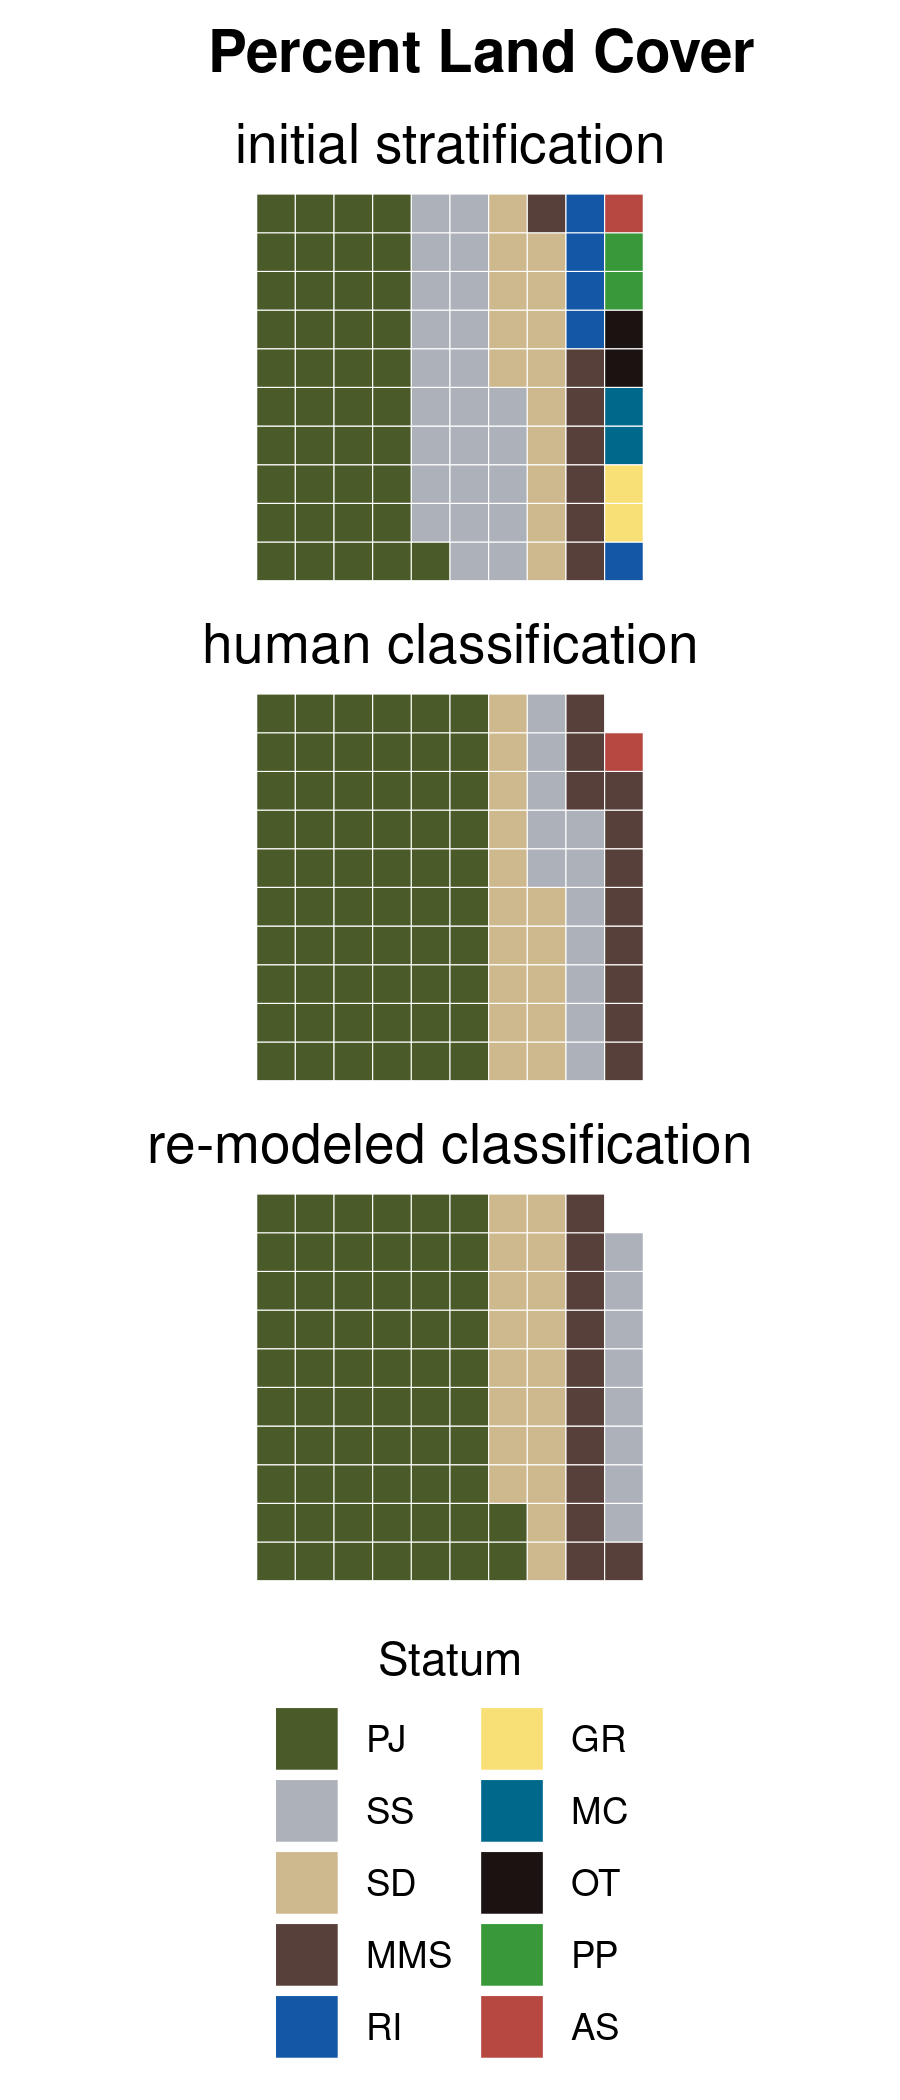
\includegraphics[width=0.5\linewidth,style="float:left; padding:10px"]{VegetationClassificationUFO_files/figure-latex/make waffle charts of changes in vegetation-1} \caption{Changes in Predicted Land Cover}\label{fig:make waffle charts of changes in vegetation}
\end{figure}

Both the total area of each vegetation type, stratum, and the number of
plots per stratum influence the statistical conclusions which can be
drawn in these areas. An increase in the surface area of a stratum,
without an increase in the number of plots would decrease the
statistical confidence associated with conclusions from it and
\emph{vice versa}. However, if the weights of point drops were
equivalent in all study areas

The initial AIM sample design was based upon a stratification which
included \texttt{r} communities. This design was based on a manual
reclassification of the GAP/LANDFIRE National Terrestrial Ecosystems
2011 data set.

\hypertarget{references}{%
\section{References}\label{references}}

\end{document}
